\documentclass[useAMS, usenatbib]{mnras}
\pdfsuppresswarningpagegroup=1
%
\usepackage[spanish,es-minimal,english]{babel}
\usepackage[utf8]{inputenc}
\usepackage{graphicx}

\usepackage{xcolor}
\usepackage{hyperref}
\usepackage{siunitx}
\usepackage{newtxtext}
\usepackage[stix2,smallerops]{newtxmath}
\usepackage{booktabs}
\hypersetup{colorlinks=True, linkcolor=blue!50!black, citecolor=black,
  urlcolor=blue!50!black}
\usepackage{etoolbox}
\robustify\bfseries
\robustify\itshape

\usepackage[shortlabels]{enumitem}

\bibliographystyle{mnras}

\sisetup{
  % explicit "+" is useful for velocities
  retain-explicit-plus = true,
  % prefer 10^6 over 1 x 10^6
  retain-unity-mantissa = false,
  % Use x +/- e instead of x(e)  
  separate-uncertainty = true,
  % Make sure to pick up bold font when used in section heading for instance
  detect-weight = true,
}
\DeclareSIUnit\msun{\text{M\ensuremath{_\odot}}}
\DeclareSIUnit\lsun{\text{L\ensuremath{_\odot}}}

%%
%% Will macros
%%
% A better \ion command that works in more circumstances
\newcommand\ION[2]{#1\,\scalebox{0.9}[0.8]{\uppercase{#2}}}
\newcounter{ionstage}
\renewcommand{\ion}[2]{\setcounter{ionstage}{#2}% 
  \ensuremath{\mathrm{#1\,\scriptstyle\Roman{ionstage}}}}
\newcommand\hii{\ion{H}{2}}
\newcommand\nii{[\ion{N}{2}]}
\newcommand\oiii{[\ion{O}{3}]}
\newcommand\oii{[\ion{O}{2}]}
\newcommand\Wav[1]{\ensuremath{\lambda #1}}
% Chemical formulae
\newcommand*\chem[1]{\ensuremath{\mathrm{#1}}}

\newcommand\Fion{\ensuremath{F_{\text{ion}}}}
\newcommand\ionpar{\ensuremath{U_{\text{ion}}}}

\title[Doubly ionized oxygen in the Orion Nebula]{
  Fluorescence versus temperature fluctuations
  in the spectrum of doubly ionized oxygen
  in the Orion Nebula
}

\author[Henney et al.]{%
  William J. Henney,\(^1\)\thanks{
    w.henney@irya.unam.mx
  }
  J. Garc{\'{\i}}a-Rojas,\(^{2,3}\)
  J. E. M\'endez-Delgado,\(^{2,3}\)
  C. Esteban,\(^{2,3}\)
  \newauthor 
  A. Mesa-Delgado,\(^{4}\)
  K. Z. Arellano-C\'ordova,\(^{2}\)
  and 
  M. Núñez-Díaz\(^{4}\)
  \\
  \(^1\)\foreignlanguage{spanish}{
    Instituto de Radioastronomía y
    Astrofísica, Universidad Nacional Autónoma de México, Apartado
    Postal 3-72, 58090 Morelia, Michaoacán, Mexico}
  \\
  \(^2\)\foreignlanguage{spanish}{
    Instituto de Astrof\'isica de Canarias (IAC), E-38205 La Laguna, Spain}
  \\
  \(^3\)\foreignlanguage{spanish}{
    Departamento de Astrof\'isica, Universidad de La Laguna, E-38206 La Laguna, Spain}
  \\
  \(^4\)\foreignlanguage{spanish}{
     Domicilio Particular, Tenerife, Spain}
}
% These dates will be filled out by the publisher
\date{Accepted XXX. Received YYY; in original form ZZZ}

% Enter the current year, for the copyright statements etc.
\pubyear{2020}

\begin{document} 
\label{firstpage}
\pagerange{\pageref{firstpage}--\pageref{lastpage}}
\maketitle

\begin{abstract}
  There are four different types of electron temperature diagnostics
  that can be derived from \ion{O}{2} recombination lines
  and [\ion{O}{3}] collisionally excited lines emitted 
  by doubly-ionized oxygen (\chem{O^{++}}) in photoionized nebulae.
  Each type of diagnostic shows a particular bias towards
  high-temperature or low-temperature regions along the line of sight.
  Differences between two or more of the diagnostics
  have traditionally been interpreted in terms of temperature fluctuations:
  either the \(t^2\) parameter or, in more extreme cases,
  the hypothesis of high-metallicity cold clumps.
  However, radiative pumping by ultraviolet starlight (fluorescence)
  of low-angular-momentum states in the \ion{O}{2} spectrum
  may potentially interfere with these diagnostics.
  Disentangling these two effects is important for the interpretation of the
  abundance discrepancy factor (ADF) in photoionized nebulae.
  We show that the spatial distribution of the \ion{O}{2} V1 multiplet
  in the Orion Nebula \ion{H}{2} region 
  is suggestive of a significant fluorescent contribution to these lines.
  Furthermore, we show that the relative ordering of temperatures
  derived from the four types of diagnostics is inconsistent with
  any form of temperature fluctuations,
  but is consistent with the effects of fluorescence.
  We conclude that fluorescence is the likely explanation
  for moderate abundance discrepancies (\(\mathrm{ADF} \approx 2\))
  observed in \ion{H}{2} regions and some planetary nebulae,
  although temperature and abundance inhomogeneities remain the favored explanation
  for the extreme abundance discrepancies (\(\mathrm{ADF} > 5\))
  seen in other planetary nebulae.
\end{abstract}


\begin{keywords}
  Atomic physics
  -- H II regions
  -- Radiative transfer
  -- techniques: imaging spectroscopy
\end{keywords}

\maketitle

\section{Introduction}
\label{sec:introduction}


\begin{figure}
  \centering
  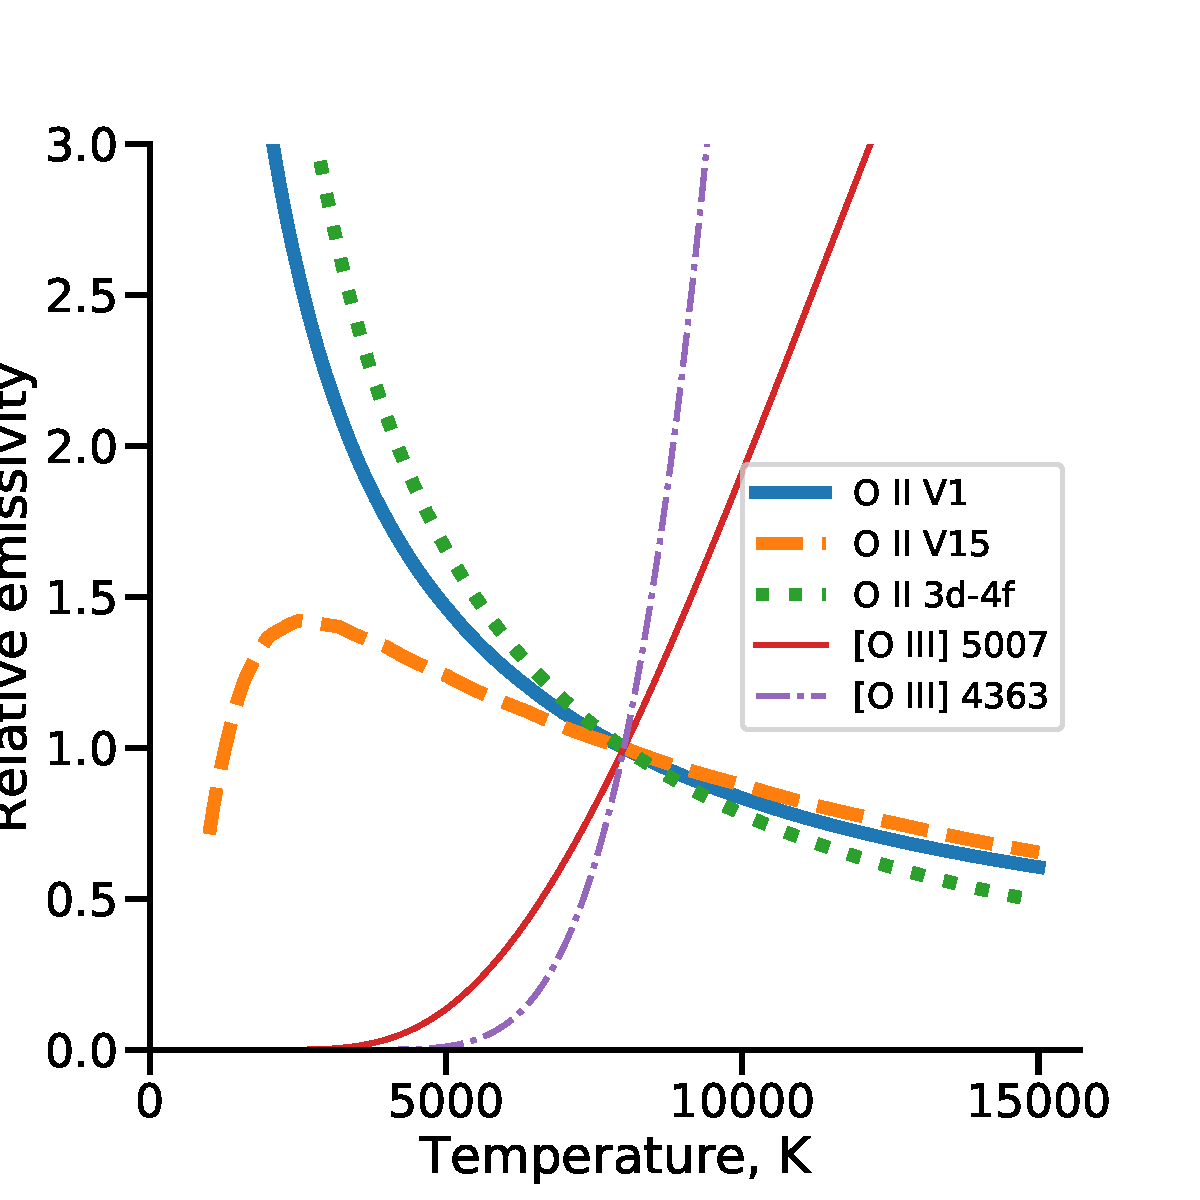
\includegraphics[width=\linewidth]{figs/oii-emissivity-vs-t}
  \caption{Emissivities of different \chem{O^{++}} lines versus temperature.}
  \label{fig:emissivities}
\end{figure}




\section{MUSE observations of Orion}
\label{sec:muse-observ-orion}

\begin{figure}
  \centering
  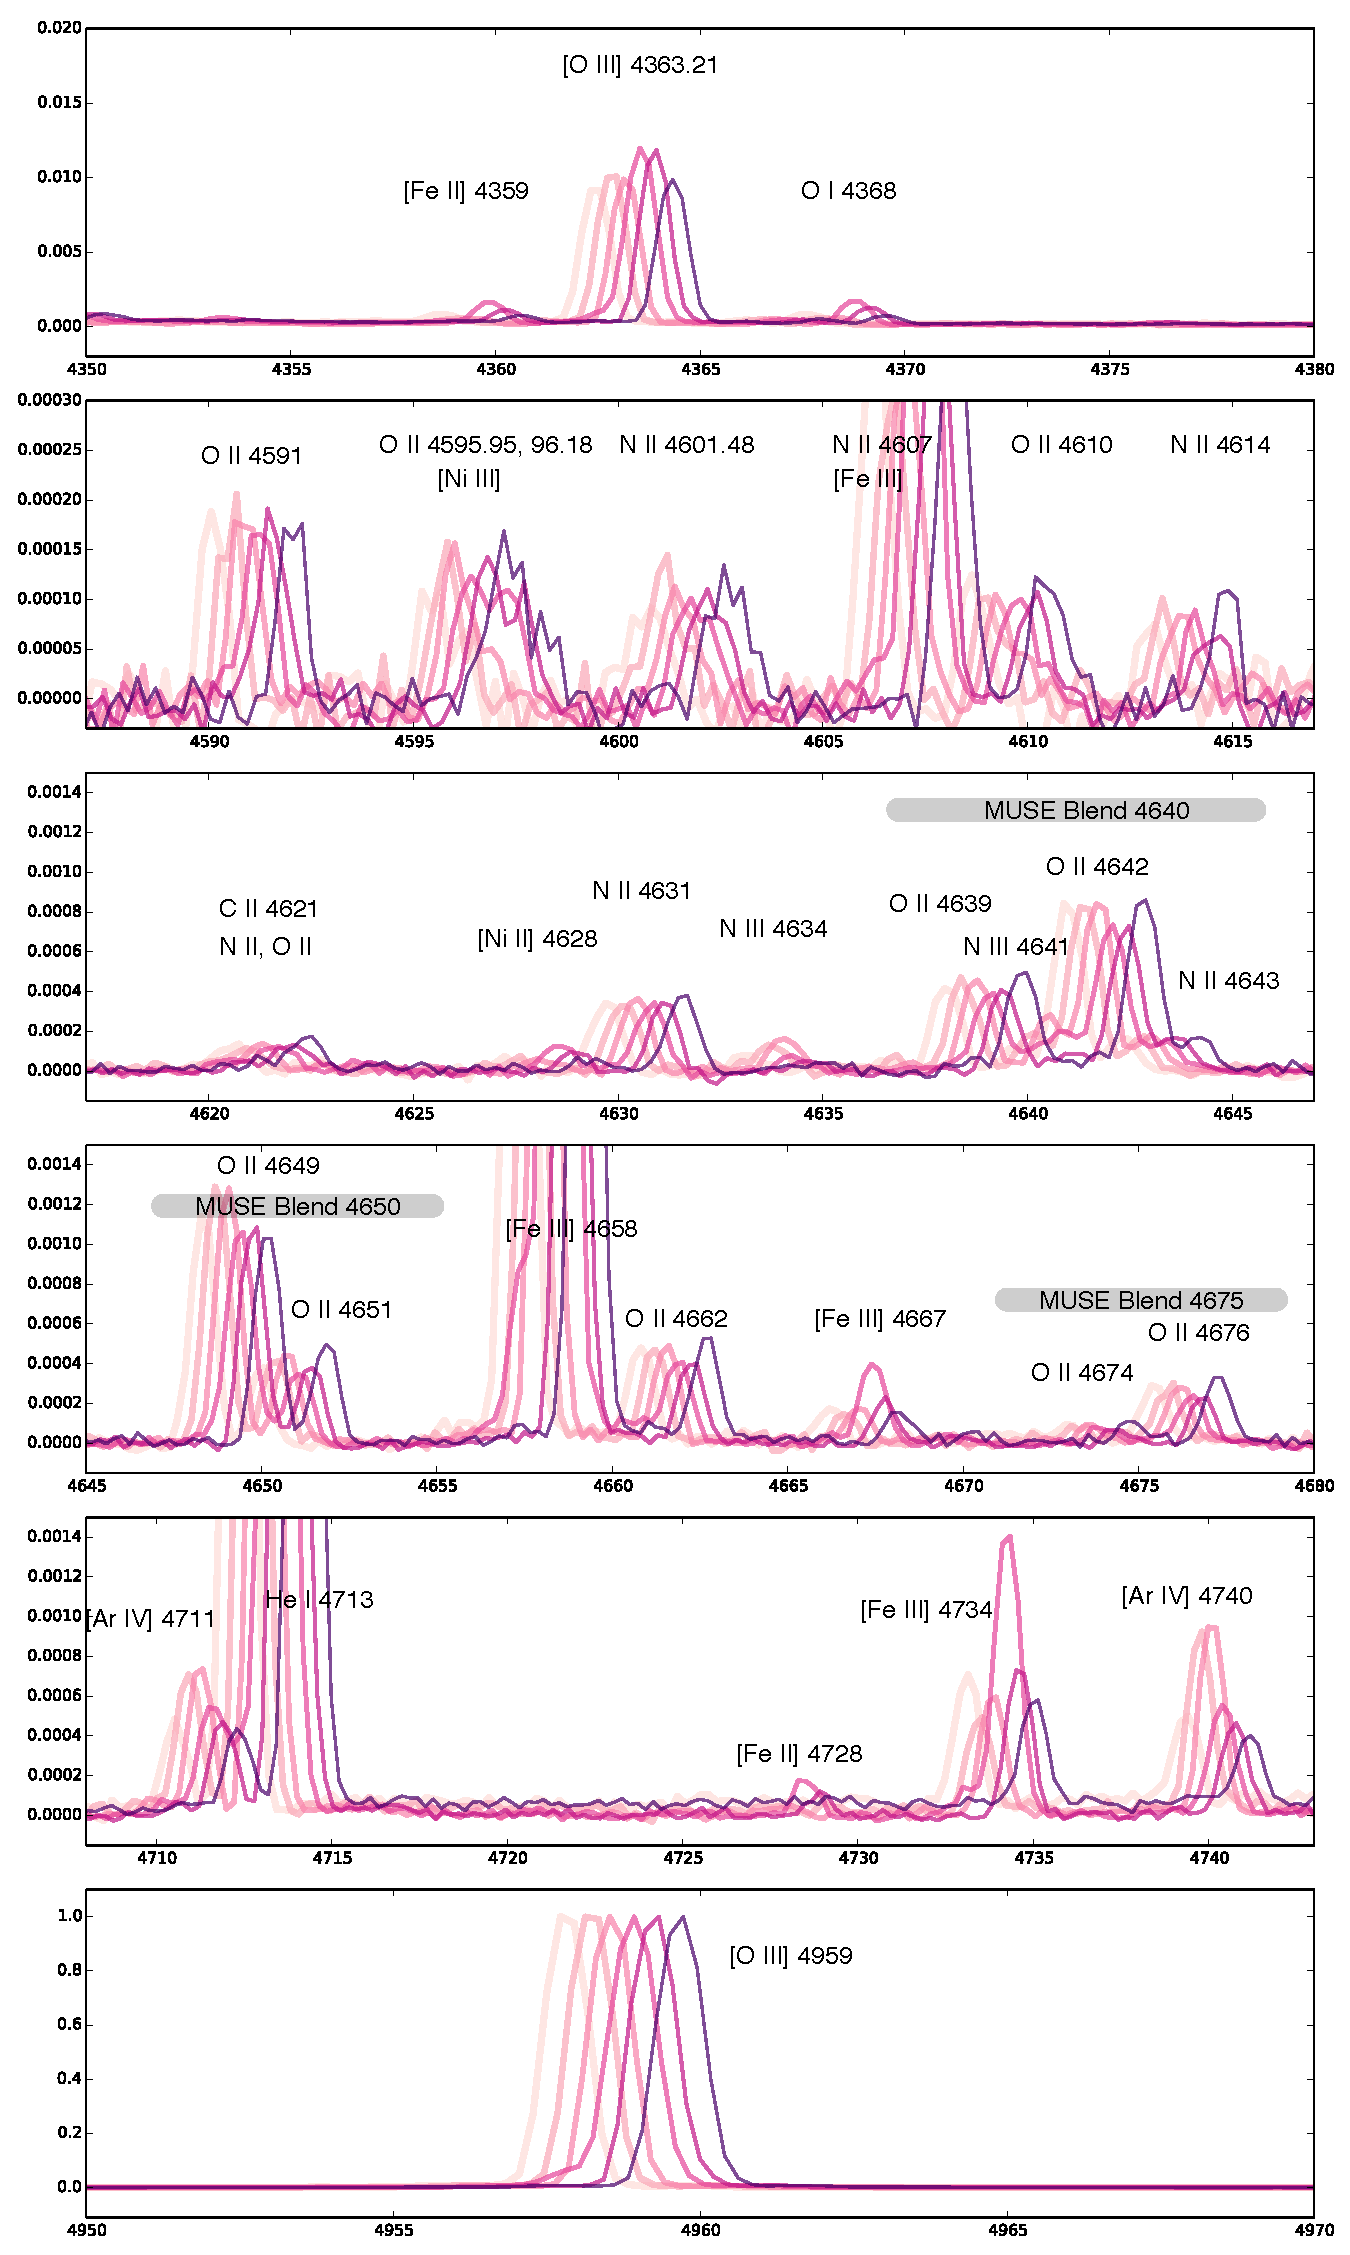
\includegraphics[width=\linewidth]{figs/adal-slit6-oii-v1-annotated}
  \caption{High-resolution ISIS-WHT spectra}
  \label{fig:adal-pink-spectra}
\end{figure}

\begin{figure*}
  \centering
  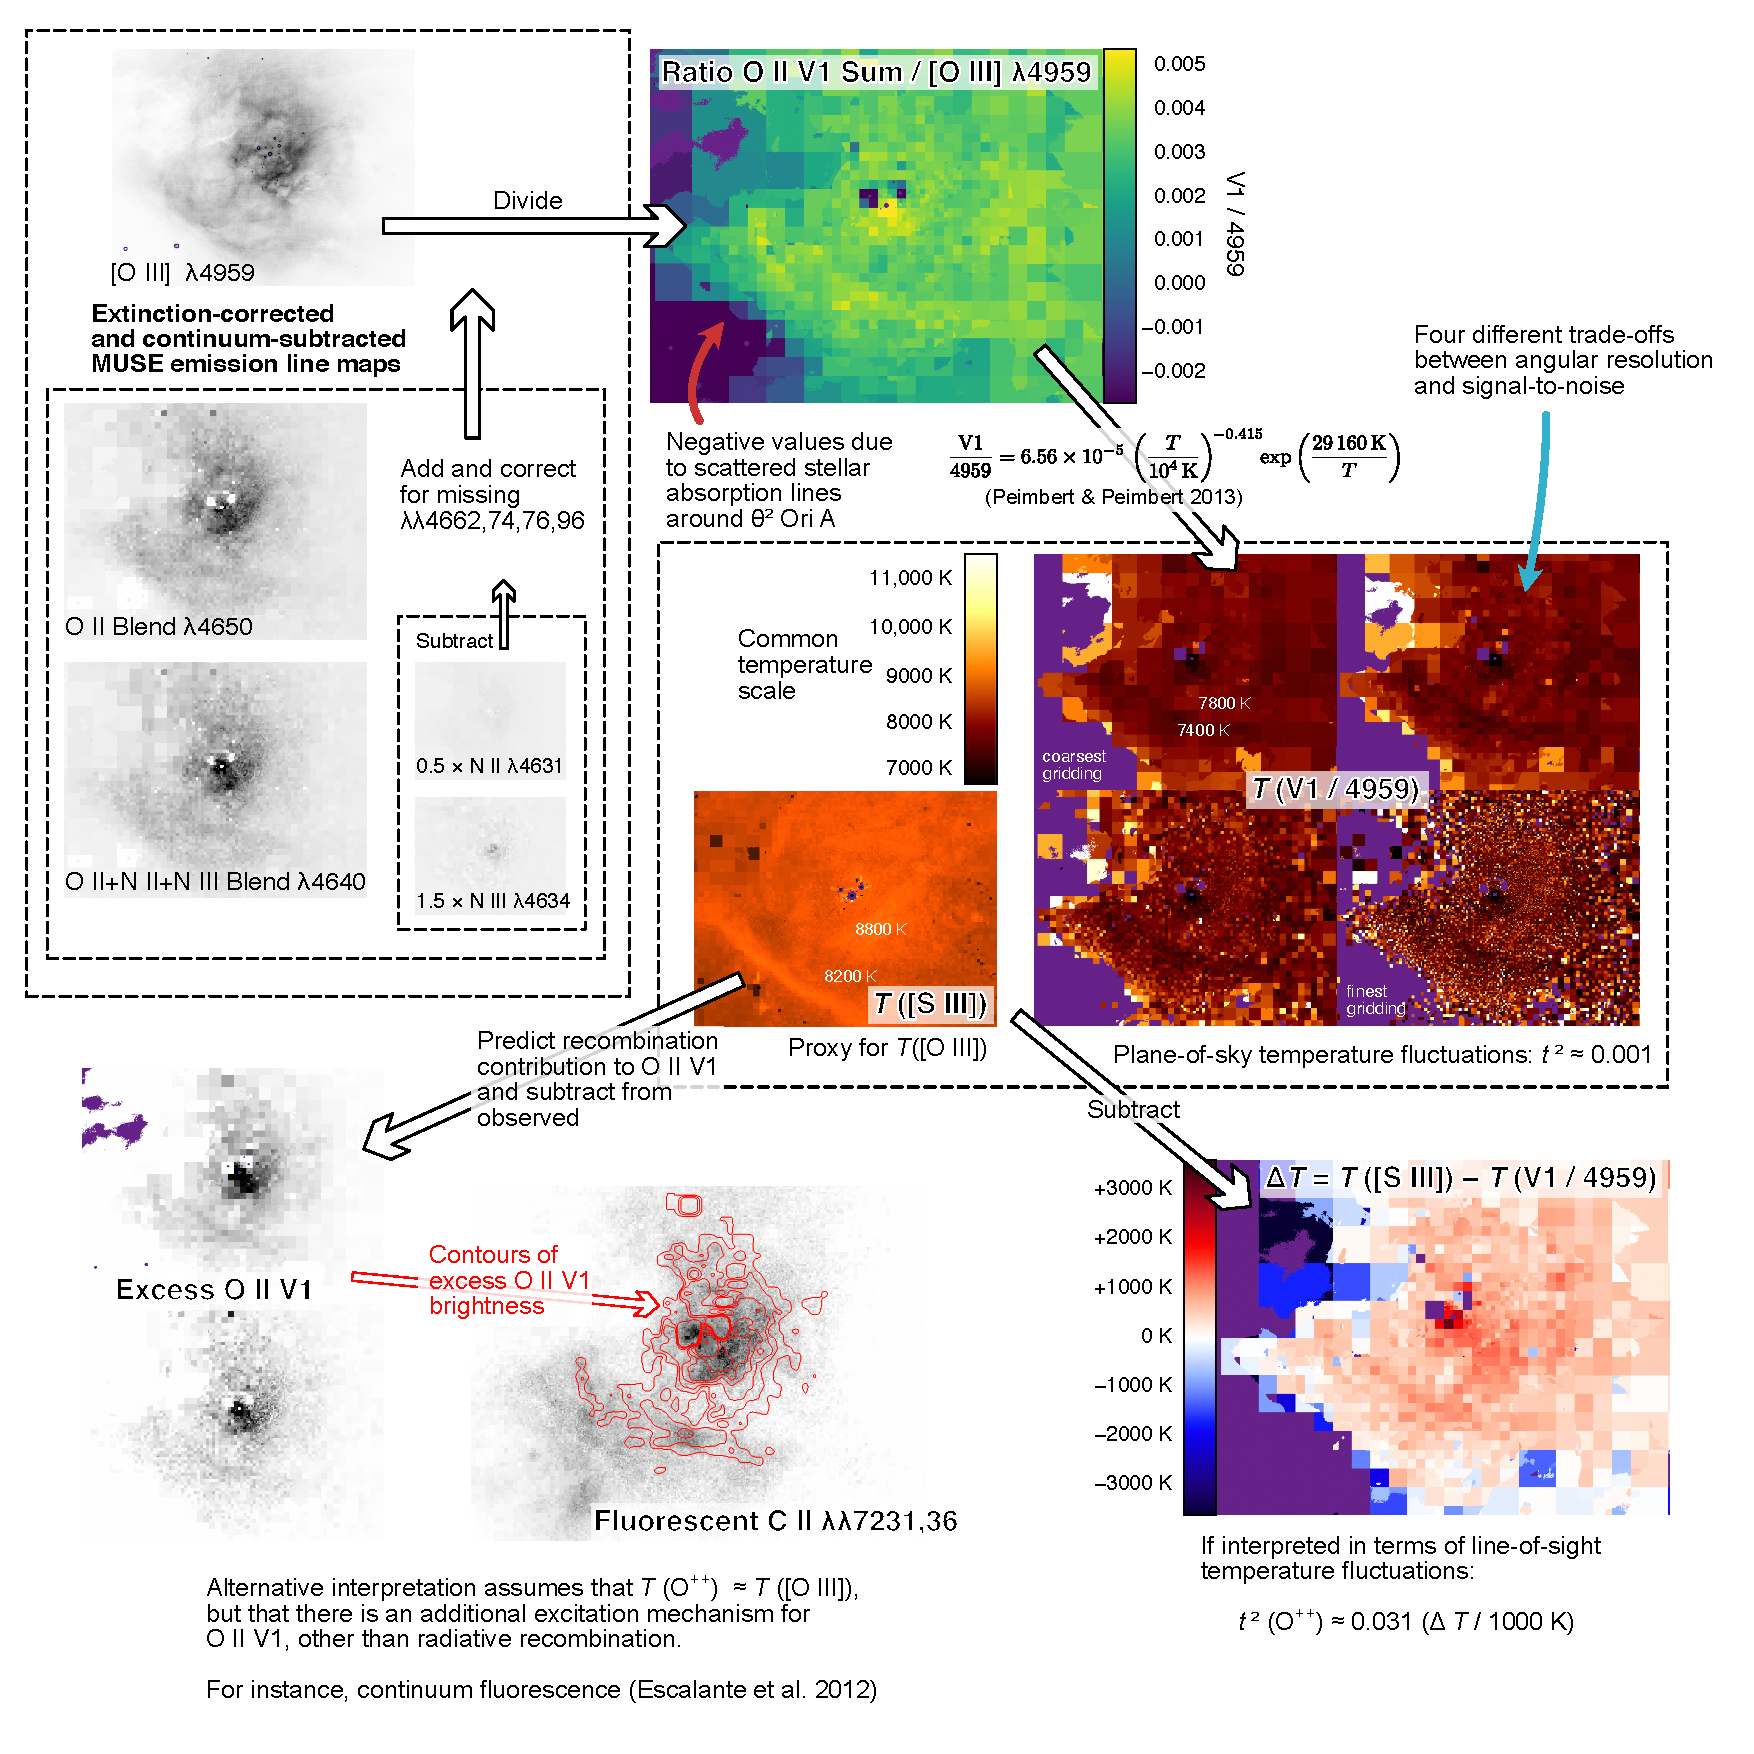
\includegraphics[width=\linewidth]{figs/oii-v1-extraction-workflow}
  \caption{Workflow for analyzing MUSE \ion{O}{2} spectral maps.  }
  \label{fig:muse-workflow}
\end{figure*}



\section{Discussion}
\label{sec:discussion}

Other \ion{H}{2} regions.

Planetary nebulae with moderate ADF.
For instance the Ring Nebula \citep{Garnett:2001a} shows \ion{O}{2}~V1 peaking just inside [\ion{O}{3}],
which is what one would expect from fluorescence. 


Planetary nebulae with high ADF.
I don't think there is any evidence for fluorescence being important in this case.
\citet{Fang:2013a} have the lowest temperatures from \ion{O}{2} 3d--4f,
which is consistent with cold clumps.

\section{Conclusions}
\label{sec:conclusions}


\bibliography{BibdeskLibrary}


% Don't change these lines
\bsp	% typesetting comment
\label{lastpage}

\end{document}


%%% Local Variables:
%%% mode: latex
%%% TeX-master: t
%%% End:
